\begin{frame}{ЭПР-парадокс}
 \begin{columns}
   \column{0.4\textwidth}
   \begin{figure}
     \includegraphics[width=\textwidth]{bi-entanglement.png}
   \end{figure}

   \column{0.5\textwidth}
   \begin{block}{}
     Работа Эйнштейна—Подольского-Розена\footnote[frame]{A. Einstein, B. Podolsky, and N. Rosen \textit{Phys. Rev.} \textbf{47}, 777 (1935)}
     указывала на неполноту квантовой механики с помощью мысленного эксперимента,
     заключающегося в измерении параметров микрообъекта косвенным образом,
     без непосредственного воздействия на этот объект.
   \end{block}
   \begin{block}{}
      В 2008 году был проведён эксперимент\footnote[frame]{T. Scheidl et al. \textit{PNAS} \textbf{107}, 46, 19708-19713 (2010)},
      который подтвердил нелокальный\footnote[frame]{J.S. Bell \textit{Physics Physique Физика} \textbf{1}, 195 (1964)}
      характер квантовой теории.
   \end{block}
 \end{columns}
\end{frame}
\note{
  В рамках теории квантовой механики, которая складвывалась в начале 20 века (1935), 
  группа авторов во главе с Эйнштейном представила некоторый класс состояний пары частиц.
  В этом состоянии измерение одной из частиц приводит к измерению другой частицы. 
  Это происходит мгновенно и не зависит от расстояния между частицами. 
  Также это можно пояснить иначе. 
  Оказывается, что в некоторых случаях невозможно разделить две частицы,
  так чтобы можно было бы работать с ними независимо.
  По мнению авторов этот результат указывал на несостоятельность текущей квантовой теории. 
  
  Через 30 лет (1964) Джон Стюарт Белл предложил эксперимент, 
  позволяющий проверить существование таких состояний. 
  Он доказал, 
  что вероятность некоторого исхода такого эксперимента не может превышать определенного значения, 
  если запутанных состояний не существует. 
  Результат этой работы часто упоминается как теорема Белла или неравенства Белла.
}

\begin{frame}{Нобелевская премия по физике 2022}
  \begin{figure}
      \centering
      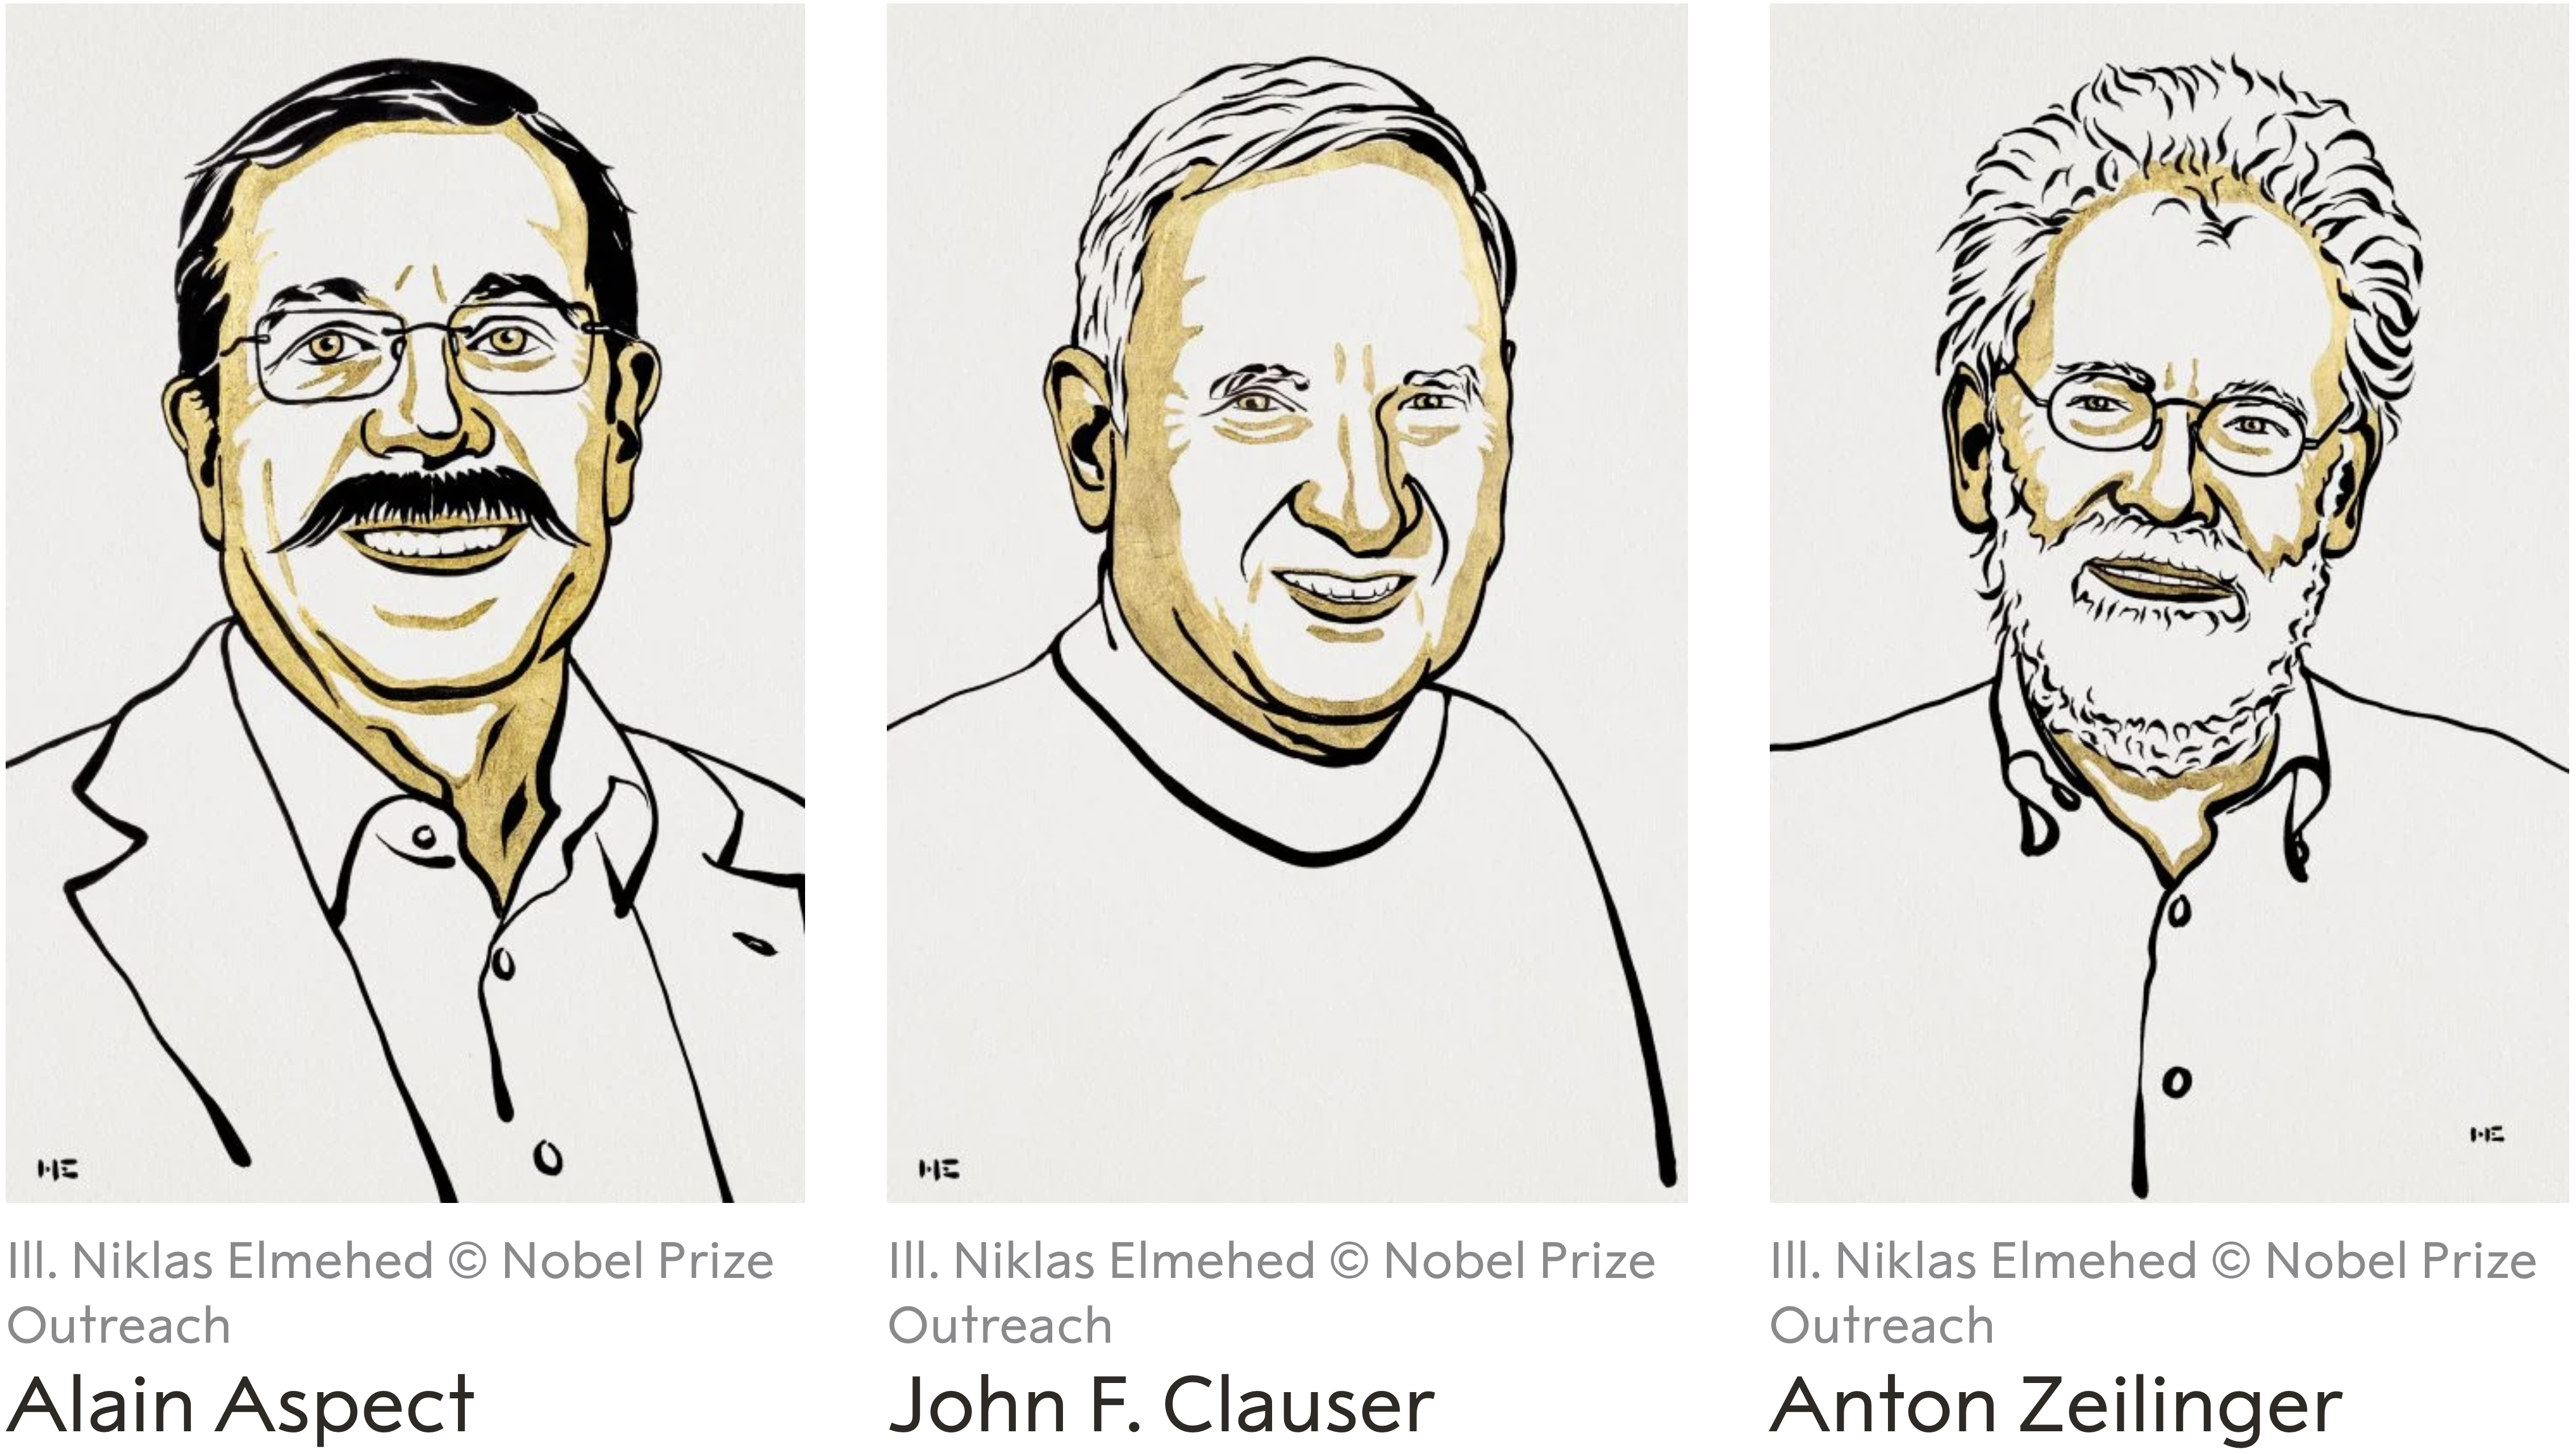
\includegraphics[width=0.8\textwidth]{nobel-prize-laureates.png}
      % \caption{Caption}
      % \label{fig:my_label}
  \end{figure}
\end{frame}
\note{
  Через несколько лет в 70 (1972) годах Джоном Клаузером и Аленом Аспе независимо были проведены первые эксперименты.
  Результаты нарушали неравенство Белла и подтверждали нелокальный характер квантовой теории.
  К оригинальным экспериментам было много вопросов,
  и авторы продолжали усложнять схему.
  
  В 2008 году группа во главе с Цайлингером провела полномаштабный эксперимент, 
  который снова подтвердил нелокальный характер квантовой теории.
  
  % Первый эксперимент был проведён Джоном Клаузером в 1972 (википедия).
  % Второй первый эксперимент был проведён Аленом Аспе в 70е.
  % (Alain Aspect Phys. Rev. D 14, 1944 – Published 15 October 1976)
  % И затем было еще много экспериментов.
  
  А буквально месяц назад произошло знаменательное событие. 
  Эта группа авторов получила нобелевскую премию по физики за эту работу. 
    
  Можно смело сказать, что в настоящее время признано, 
  что запутанность является ключевой концепцией квантовой теории. 
}

\begin{frame}{Приложения запутанности}
  \begin{columns}
    \column{0.6\textwidth}
    \begin{figure}
        \centering
        \includegraphics[width=\textwidth]{Kaufman2016-quanty-quench.png}
        \caption{Science, 353(6301):794-800 (2016)}
        %\label{fig:my_label}
    \end{figure}
    \column{0.4\textwidth}
    \begin{figure}
       \includegraphics[width=0.8\textwidth]{sycamore-supemancy.png}
       % \captionsetup{labelformat=empty}
       \caption{
         % F. Arute et al., Nature 574, 505 (2019)
         Nature 574, 505 (2019)
       }
    \end{figure}
  \end{columns}
\end{frame}
\note{
    Cегодня поднимаются вопросы о о квантовом превосходстве, 
    как в работе группы Мартинеса, 
    или исследованиях проблемы термализации, 
    как в работе группы Маркуса Грайнера (Greiner),
    где мы имеем многочастичную систему. 
    Поэтому особый интерес вызывает многочастичная запутанность,
    а не парная.
    
    В последние годы возникли методы исследования многочастичной запутанности.
    В частности, оказалось, что в рамках многоквантовой (МК) спектроскопии ЯМР в твердом теле можно существенно продвинуться в этом направлении.

    Это является главной мотивацией данной диссертации. 
}

\begin{frame}{Цели и задачи}
  \textbf{Целью данной работы} является теоретическое исследование многочастичной запутанности в системах с большим количеством частиц (>200) в рамках МК спектроскопии ЯМР,
а также развитие методов экспериментального измерения величин квантовой информации Фишера и косой информации Вигнера-Янасе.
\end{frame}
\note{
  Целью данной работы является...
}

\begin{frame}{Положения, выносимые на защиту}
  \begin{enumerate}
  \item
  Разработанная теория МК ЯМР позволяет исследовать многочастичную запутанность в системе ядерных спинов при произвольной температуре.

  \item
  С понижением температуры количество запутанных спинов растет и в нанопоре, и в зигзагобразной цепочке. 
  % В нанопоре, заполненой спин несущими частицами, при температуре 
  % $T = 6.856\cdot10^{-3}$~K $(\beta=3.5)$ 
  % почти все спины (до 179 из 201) запутаны.
  %Исследована температурная зависимость многочастичной запутанности в нанопоре,
  %когда система приготовлена в термодинамическом равновесном зеемановском и дипольном упорядоченном состояниях.

  \item
  Оценка количества запутанных спинов в однородных цепочках согласуется с результатами, представленными в литературе.
  % Исследована многочастичная запутанность в квазиодномерных цепочках ядерных спинов в зависимости от параметров цепи и температуры.

  \item
  Если спиновая система исследуется в МК эксперименте ЯМР с начальным равновесным термодинамическим состоянием при температуре $T$, 
  то ее косая информация Вигнера-Янасе равна удвоенному второму моменту распределения интенсивностей МК когерентностей ЯМР системы, приготовленной при вдвое большей температуре $2T$ в тот же момент времени эволюции;
  % Предложен метод экспериментального измерения точного значения косой информации Вигнера-Янасе в рамках МК спектроскопии ЯМР.

  \item
  Результаты оценки количества запутанных спинов, полученные на основе квантовой информации Фишера и косой информации Вигнера-Янасе, согласуются;
  % Проведено сравнение оценок многочастичной запутанности, 
  % полученных на основе квантовой информации Фишера и косой информации Вигнера-Янасе.
\end{enumerate}

\end{frame}
\note{
    На защиту выносятся следующие положения...
}

\begin{frame}{Научная новизна и практическая ценность}
  \begin{block}{Научная новизна.}
    В данной работе была разработана теория МК ЯМР для нанопоры~\cite{Doronin2019} при произвольной температуре,
что позволило впервые теоретически исследовать температурную зависимость многочастичной запутанности в системе из более чем 200 взаимодействующих частиц~\cite{Doronin2019, Lazarev2020}.
Также в данной работе был разработан~\cite{Doronin2021} метод определения величины косой информации Вигнера-Янасе в МК эксперименте ЯМР.
  \end{block}

  \begin{block}{Практическая ценность.}
   Так как косая информация Вигнера-Янасе нашла много применений в квантовой теории информации, %~\cite{Wigner1963, Luo2017},
предлагаемый в данной работе метод определения ее величины
не только позволяет~\cite{Doronin2021} исследовать многочастичную запутанность методами МК ЯМР,
но и открывает возможность решения широкого класса задач в этой области.
  \end{block}
\end{frame}